\documentclass[11pt]{article}
\usepackage[margin=0.75in]{geometry}
\usepackage{amsmath}
\usepackage{amssymb}
\usepackage{enumitem}
\usepackage{xcolor}
\usepackage{tikz}
\usepackage{pgfplots}
\pgfplotsset{compat=1.18}
\usepackage{tcolorbox}
\usepackage{graphicx}
\usepackage{multicol}

% Custom boxes
\newtcolorbox{intuition}{colback=blue!5!white,colframe=blue!75!black,title=\textbf{Intuition}}
\newtcolorbox{example}{colback=green!5!white,colframe=green!75!black,title=\textbf{Example}}
\newtcolorbox{warning}{colback=red!5!white,colframe=red!75!black,title=\textbf{Common Mistake}}
\newtcolorbox{steps}{colback=yellow!5!white,colframe=orange!75!black,title=\textbf{How to Solve}}

\title{\textbf{ECO310 Midterm 1: Intuitive Study Guide}}
\date{}

\begin{document}
\maketitle

\section{Consumer Preferences: What People Want}

\subsection{The Big Picture}
Economics starts with a simple question: \textit{How do people choose?} We need to model how consumers rank different bundles of goods.

\begin{intuition}
Think of it like ranking your favorite meals. You might prefer pizza over salad, salad over plain bread, etc. If your preferences are "rational," you can consistently rank any two options and those rankings don't contradict each other.
\end{intuition}

\subsection{Indifference Curves: Your Preference Map}

\begin{center}
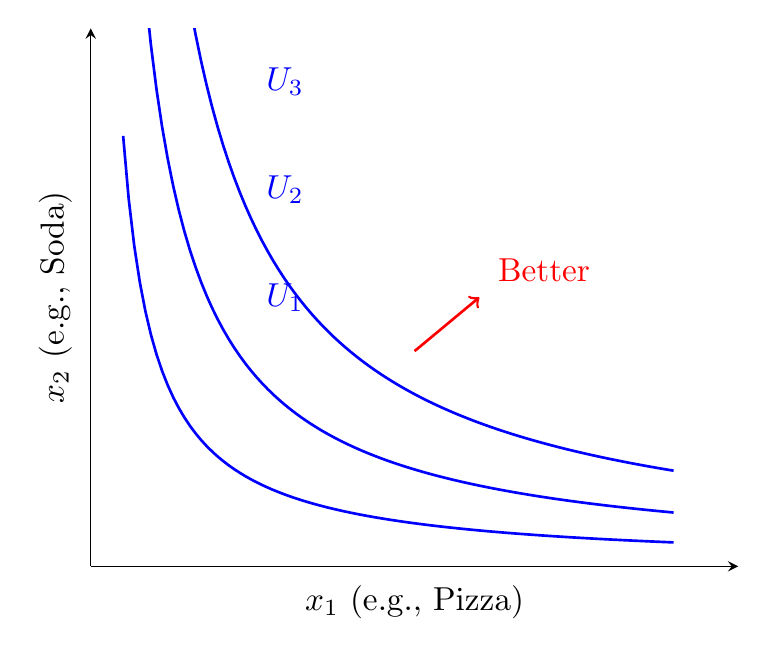
\begin{tikzpicture}[scale=1.2]
\begin{axis}[
    axis lines=left,
    xlabel={$x_1$ (e.g., Pizza)},
    ylabel={$x_2$ (e.g., Soda)},
    xmin=0, xmax=10,
    ymin=0, ymax=10,
    xtick=\empty,
    ytick=\empty,
    domain=0.5:9,
    samples=100
]
\addplot[blue, thick] {4/x};
\addplot[blue, thick] {9/x};
\addplot[blue, thick] {16/x};
\node[blue] at (axis cs:3,5) {$U_1$};
\node[blue] at (axis cs:3,7) {$U_2$};
\node[blue] at (axis cs:3,9) {$U_3$};
\draw[->,thick,red] (axis cs:5,4) -- (axis cs:6,5);
\node[red] at (axis cs:7,5.5) {Better};
\end{axis}
\end{tikzpicture}
\end{center}

\begin{intuition}
An indifference curve shows all bundles that give you the \textbf{same happiness}. Higher curves = more happiness. The curves are smooth (no jumps) and bow inward (you like variety - having some of both goods is better than lots of one).
\end{intuition}

\subsection{MRS: The Trade-Off Rate}

\textbf{Marginal Rate of Substitution (MRS)} = How many units of $x_2$ you'd give up for one more $x_1$, while staying equally happy.

\begin{center}
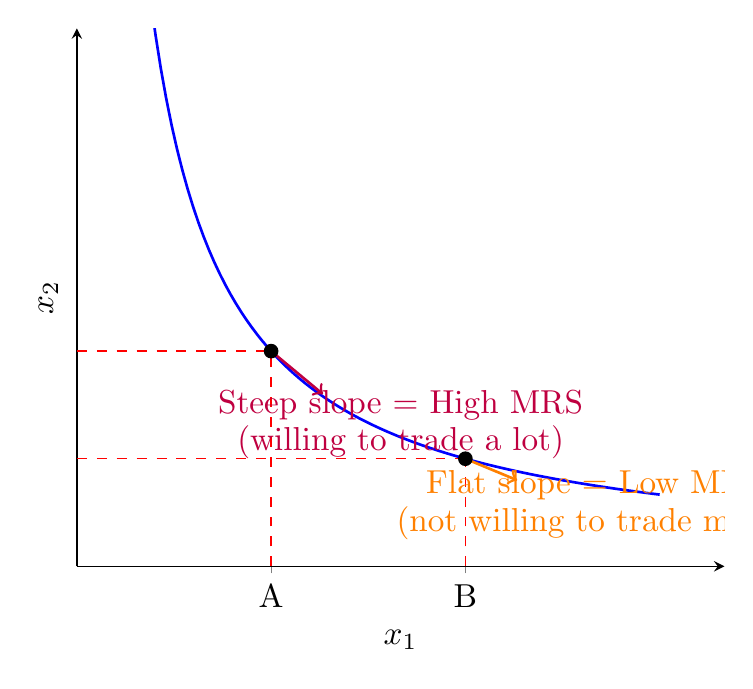
\begin{tikzpicture}[scale=1.2]
\begin{axis}[
    axis lines=left,
    xlabel={$x_1$},
    ylabel={$x_2$},
    xmin=0, xmax=10,
    ymin=0, ymax=10,
    xtick={3,6},
    xticklabels={A,B},
    ytick=\empty,
    domain=0.8:9,
    samples=100
]
\addplot[blue, thick] {12/x};
\addplot[dashed, red] coordinates {(3,0) (3,4)};
\addplot[dashed, red] coordinates {(0,4) (3,4)};
\addplot[dashed, red] coordinates {(6,0) (6,2)};
\addplot[dashed, red] coordinates {(0,2) (6,2)};
\draw[->,thick,purple] (axis cs:3,4) -- (axis cs:3.8,3.2);
\node[purple] at (axis cs:5,3) {Steep slope = High MRS};
\node[purple] at (axis cs:5,2.3) {(willing to trade a lot)};
\draw[->,thick,orange] (axis cs:6,2) -- (axis cs:6.8,1.6);
\node[orange] at (axis cs:8,1.5) {Flat slope = Low MRS};
\node[orange] at (axis cs:8,0.8) {(not willing to trade much)};
\filldraw (axis cs:3,4) circle (2pt);
\filldraw (axis cs:6,2) circle (2pt);
\end{axis}
\end{tikzpicture}
\end{center}

\textbf{Formula:} $MRS = \frac{MU_1}{MU_2}$ (ratio of marginal utilities)

\begin{intuition}
At point A, you have little pizza and lots of soda. You'd happily trade lots of soda for one more pizza (steep slope). At point B, you have more pizza, so you're less desperate - you'd only give up a little soda (flat slope). This is \textbf{diminishing MRS}.
\end{intuition}

\section{Budget Constraints: What You Can Afford}

\subsection{The Budget Line}

You have income $m$ and face prices $p_1, p_2$. Your budget constraint:
$$p_1 x_1 + p_2 x_2 = m$$

\begin{center}
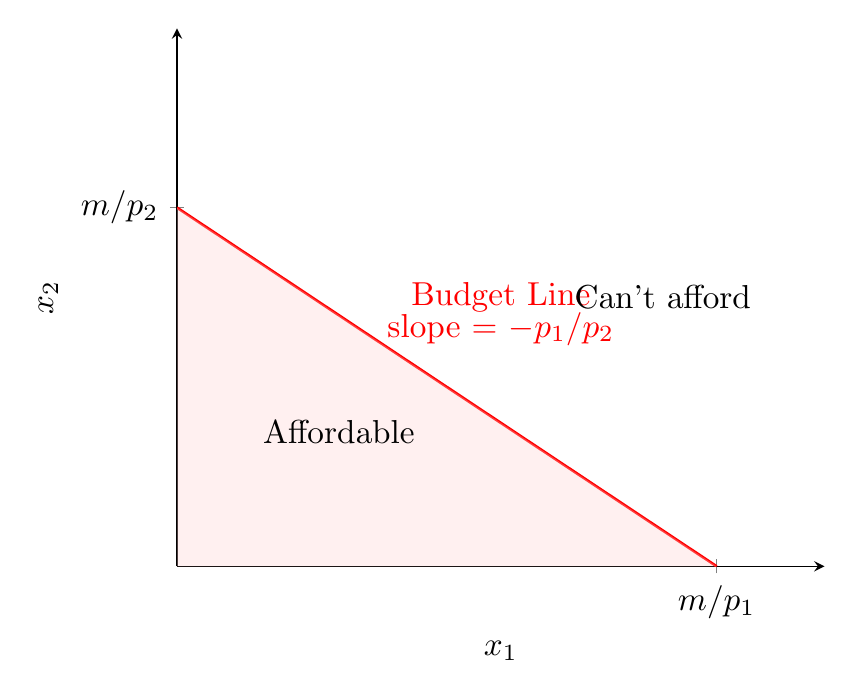
\begin{tikzpicture}[scale=1.2]
\begin{axis}[
    axis lines=left,
    xlabel={$x_1$},
    ylabel={$x_2$},
    xmin=0, xmax=12,
    ymin=0, ymax=12,
    xtick={10},
    xticklabels={$m/p_1$},
    ytick={8},
    yticklabels={$m/p_2$},
]
\addplot[red, thick] coordinates {(0,8) (10,0)};
\fill[red!20, opacity=0.3] (axis cs:0,0) -- (axis cs:0,8) -- (axis cs:10,0) -- cycle;
\node[red] at (axis cs:6,6) {Budget Line};
\node[red] at (axis cs:6,5.3) {slope = $-p_1/p_2$};
\node at (axis cs:3,3) {Affordable};
\node at (axis cs:9,6) {Can't afford};
\end{axis}
\end{tikzpicture}
\end{center}

\begin{intuition}
The budget line shows all bundles you can \textbf{exactly} afford. The slope tells you the market trade-off: to buy one more $x_1$, you must give up $p_1/p_2$ units of $x_2$. The shaded triangle is everything you can afford.
\end{intuition}

\subsection{What Happens When Things Change?}

\begin{center}
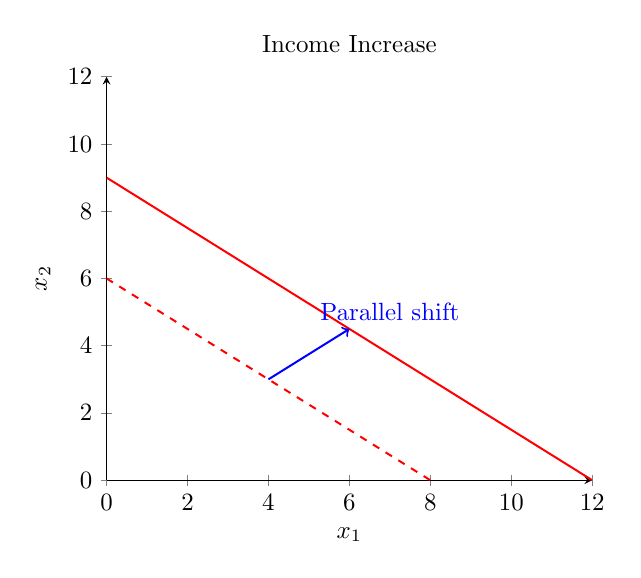
\begin{tikzpicture}[scale=0.9]
\begin{axis}[
    axis lines=left,
    xlabel={$x_1$},
    ylabel={$x_2$},
    xmin=0, xmax=12,
    ymin=0, ymax=12,
    title={Income Increase},
]
\addplot[red, thick, dashed] coordinates {(0,6) (8,0)};
\addplot[red, thick] coordinates {(0,9) (12,0)};
\draw[->,thick,blue] (axis cs:4,3) -- (axis cs:6,4.5);
\node[blue] at (axis cs:7,5) {Parallel shift};
\end{axis}
\end{tikzpicture}
\hspace{0.5cm}
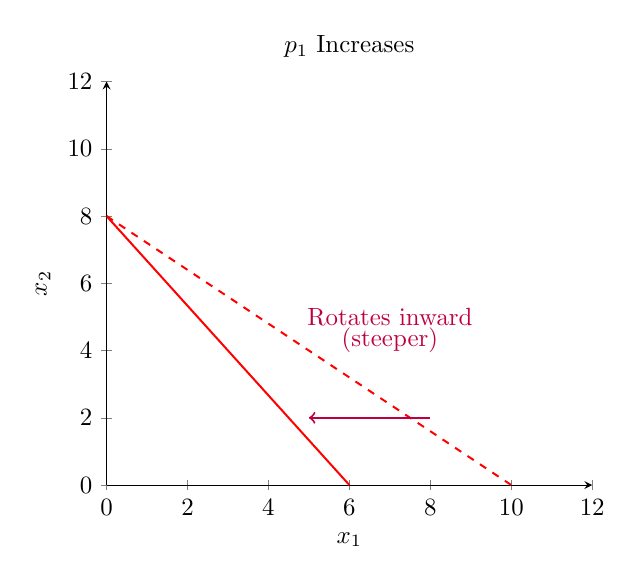
\begin{tikzpicture}[scale=0.9]
\begin{axis}[
    axis lines=left,
    xlabel={$x_1$},
    ylabel={$x_2$},
    xmin=0, xmax=12,
    ymin=0, ymax=12,
    title={$p_1$ Increases},
]
\addplot[red, thick, dashed] coordinates {(0,8) (10,0)};
\addplot[red, thick] coordinates {(0,8) (6,0)};
\draw[->,thick,purple] (axis cs:8,2) -- (axis cs:5,2);
\node[purple] at (axis cs:7,5) {Rotates inward};
\node[purple] at (axis cs:7,4.3) {(steeper)};
\end{axis}
\end{tikzpicture}
\end{center}

\section{Optimal Choice: Where to Shop}

\subsection{The Tangency Condition}

\textbf{Your goal:} Reach the highest indifference curve you can afford.

\begin{center}
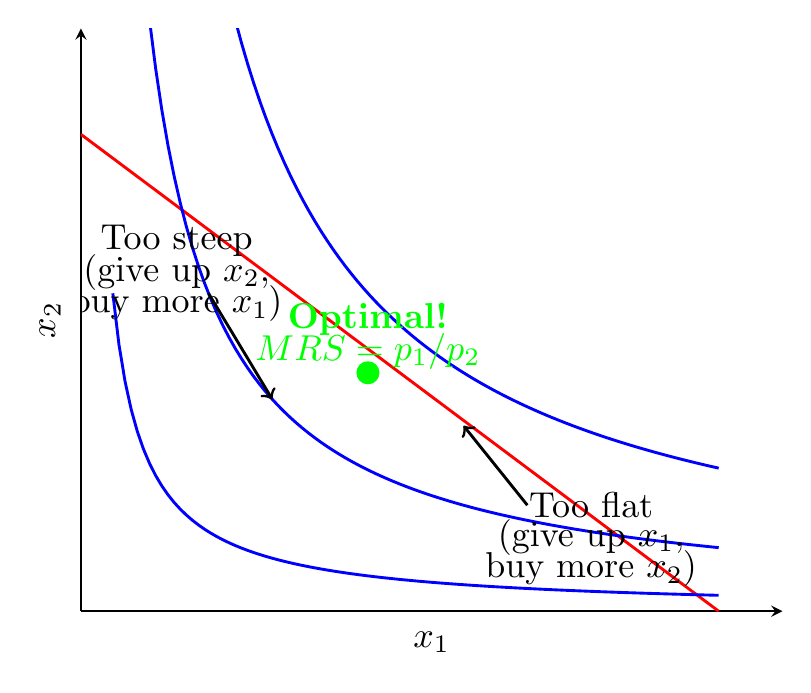
\begin{tikzpicture}[scale=1.3]
\begin{axis}[
    axis lines=left,
    xlabel={$x_1$},
    ylabel={$x_2$},
    xmin=0, xmax=11,
    ymin=0, ymax=11,
    xtick=\empty,
    ytick=\empty,
    domain=0.5:10,
    samples=100
]
\addplot[red, thick] coordinates {(0,9) (10,0)};
\addplot[blue, thick] {3/x};
\addplot[blue, thick] {12/x};
\addplot[blue, thick] {27/x};
\filldraw[green] (axis cs:4.5,4.5) circle (3pt);
\node[green] at (axis cs:4.5,5.5) {\textbf{Optimal!}};
\node[green] at (axis cs:4.5,4.9) {$MRS = p_1/p_2$};
\draw[->,thick] (axis cs:2,6) -- (axis cs:3,4);
\node at (axis cs:1.5,7) {Too steep};
\node at (axis cs:1.5,6.4) {(give up $x_2$,};
\node at (axis cs:1.5,5.8) {buy more $x_1$)};
\draw[->,thick] (axis cs:7,2) -- (axis cs:6,3.5);
\node at (axis cs:8,2) {Too flat};
\node at (axis cs:8,1.4) {(give up $x_1$,};
\node at (axis cs:8,0.8) {buy more $x_2$)};
\end{axis}
\end{tikzpicture}
\end{center}

\begin{steps}
\textbf{How to find optimal consumption:}
\begin{enumerate}[leftmargin=*]
    \item Write down utility function and budget constraint
    \item Calculate MRS = $MU_1/MU_2$ by taking derivatives
    \item Set $MRS = p_1/p_2$ (tangency condition)
    \item Plug into budget constraint: $p_1 x_1 + p_2 x_2 = m$
    \item Solve the two equations for $x_1^*$ and $x_2^*$
    \item Check: Are both positive? If not, you have a corner solution!
\end{enumerate}
\end{steps}

\begin{example}
\textbf{Problem:} $u = x_1^{0.5} x_2^{0.5}$, $p_1 = 2$, $p_2 = 4$, $m = 120$

\textbf{Solution:}
\begin{enumerate}
    \item $MU_1 = 0.5 x_1^{-0.5} x_2^{0.5}$, $MU_2 = 0.5 x_1^{0.5} x_2^{-0.5}$
    \item $MRS = \frac{MU_1}{MU_2} = \frac{x_2}{x_1}$
    \item Set $\frac{x_2}{x_1} = \frac{p_1}{p_2} = \frac{2}{4} = \frac{1}{2}$
    \item So $x_2 = \frac{1}{2}x_1$
    \item Plug into budget: $2x_1 + 4(\frac{1}{2}x_1) = 120$
    \item $4x_1 = 120 \Rightarrow x_1^* = 30$
    \item $x_2^* = \frac{1}{2}(30) = 15$
\end{enumerate}
\textbf{Answer:} Buy 30 units of good 1 and 15 units of good 2.
\end{example}

\section{Special Utility Functions: Shortcuts}

\subsection{Cobb-Douglas: The "Spend a Fraction" Rule}

$$u = x_1^a x_2^b$$

\begin{intuition}
This is the most common utility function. The magic rule: spend fraction $\frac{a}{a+b}$ of your income on good 1, and $\frac{b}{a+b}$ on good 2. \textbf{Always!} (Doesn't matter what prices are!)
\end{intuition}

\textbf{Demand formulas:}
$$x_1^* = \frac{a}{a+b} \cdot \frac{m}{p_1}, \quad x_2^* = \frac{b}{a+b} \cdot \frac{m}{p_2}$$

\begin{example}
$u = x_1^{0.3} x_2^{0.7}$, any prices, income $m = 100$

Spend $\frac{0.3}{1.0} = 30\%$ on good 1, $70\%$ on good 2.

If $p_1 = 5$: $x_1^* = \frac{30}{5} = 6$

If $p_2 = 2$: $x_2^* = \frac{70}{2} = 35$
\end{example}

\subsection{Perfect Complements: The "Bundle" Rule}

$$u = \min\{ax_1, bx_2\}$$

\begin{center}
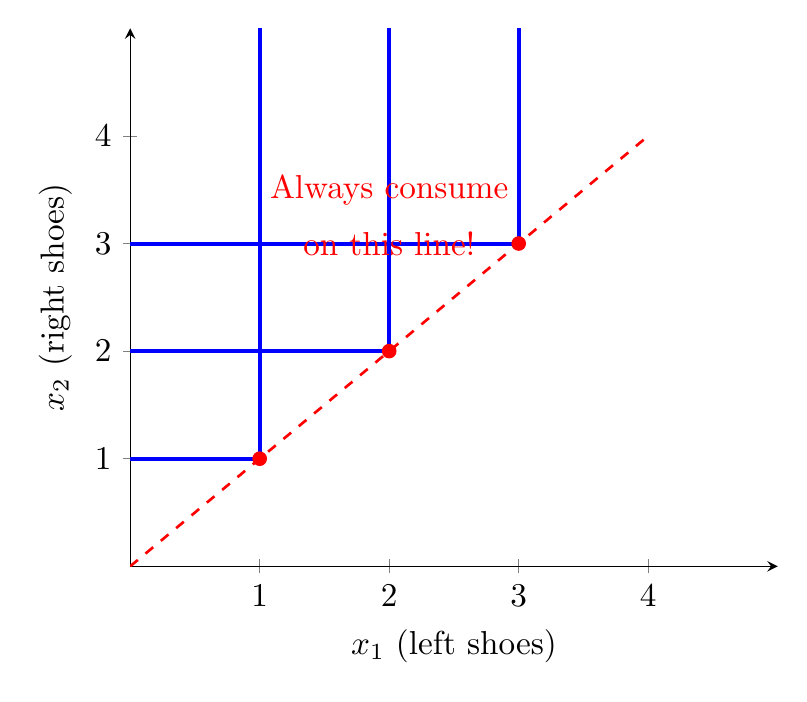
\begin{tikzpicture}[scale=1.2]
\begin{axis}[
    axis lines=left,
    xlabel={$x_1$ (left shoes)},
    ylabel={$x_2$ (right shoes)},
    xmin=0, xmax=5,
    ymin=0, ymax=5,
    xtick={1,2,3,4},
    ytick={1,2,3,4},
]
\addplot[blue, very thick] coordinates {(0,1) (1,1)};
\addplot[blue, very thick] coordinates {(1,1) (1,5)};
\addplot[blue, very thick] coordinates {(0,2) (2,2)};
\addplot[blue, very thick] coordinates {(2,2) (2,5)};
\addplot[blue, very thick] coordinates {(0,3) (3,3)};
\addplot[blue, very thick] coordinates {(3,3) (3,5)};
\filldraw[red] (axis cs:1,1) circle (2pt);
\filldraw[red] (axis cs:2,2) circle (2pt);
\filldraw[red] (axis cs:3,3) circle (2pt);
\draw[red, thick, dashed] (axis cs:0,0) -- (axis cs:4,4);
\node[red] at (axis cs:2,3.5) {Always consume};
\node[red] at (axis cs:2,3) {on this line!};
\end{axis}
\end{tikzpicture}
\end{center}

\begin{intuition}
Goods are consumed in fixed proportions (like left and right shoes). Extra of one is useless. The L-shaped curves show you don't care about having 5 left shoes if you only have 1 right shoe.
\end{intuition}

\begin{steps}
\textbf{How to solve:}
\begin{enumerate}
    \item Always consume at the kink: $ax_1 = bx_2$
    \item Plug into budget: $p_1 x_1 + p_2 x_2 = m$
    \item Solve for $x_1^*$ and $x_2^*$
\end{enumerate}
\end{steps}

\begin{example}
$u = \min\{x_1, 2x_2\}$ (need 2 units of $x_2$ for each $x_1$)

At kink: $x_1 = 2x_2$, so $x_2 = \frac{x_1}{2}$

Budget: $p_1 x_1 + p_2(\frac{x_1}{2}) = m$

$x_1^*(p_1 + \frac{p_2}{2}) = m$

$x_1^* = \frac{m}{p_1 + p_2/2}$, $x_2^* = \frac{m}{2p_1 + p_2}$
\end{example}

\subsection{Perfect Substitutes: The "All or Nothing" Rule}

$$u = ax_1 + bx_2$$

\begin{center}
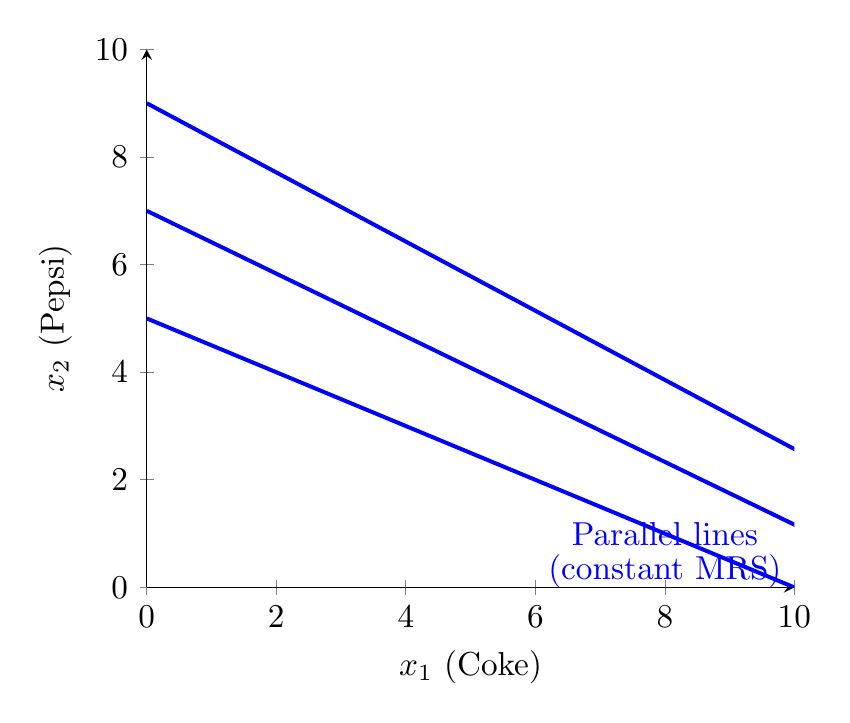
\begin{tikzpicture}[scale=1.2]
\begin{axis}[
    axis lines=left,
    xlabel={$x_1$ (Coke)},
    ylabel={$x_2$ (Pepsi)},
    xmin=0, xmax=10,
    ymin=0, ymax=10,
]
\addplot[blue, very thick] coordinates {(0,5) (10,0)};
\addplot[blue, very thick] coordinates {(0,7) (12,0)};
\addplot[blue, very thick] coordinates {(0,9) (14,0)};
\node[blue] at (axis cs:8,1) {Parallel lines};
\node[blue] at (axis cs:8,0.3) {(constant MRS)};
\end{axis}
\end{tikzpicture}
\end{center}

\begin{intuition}
Goods are perfect substitutes (like Coke vs Pepsi to someone who doesn't care). The indifference curves are straight lines. You'll buy ALL of whichever is cheaper per unit of utility.
\end{intuition}

\begin{steps}
\textbf{Decision rule:}
\begin{itemize}
    \item If $\frac{a}{p_1} > \frac{b}{p_2}$: good 1 gives more "bang per buck" $\Rightarrow$ buy only $x_1 = m/p_1$
    \item If $\frac{a}{p_1} < \frac{b}{p_2}$: good 2 is better $\Rightarrow$ buy only $x_2 = m/p_2$
    \item If equal: you're indifferent, buy any combination on the budget line
\end{itemize}
\end{steps}

\subsection{Quasilinear: The "No Income Effect" Function}

$$u = v(x_1) + x_2$$

\begin{intuition}
Good 2 is like "money" - you always want more of it, but it doesn't affect how you value good 1. Your demand for good 1 depends \textbf{only on its price}, not your income (as long as you have enough income to afford some of both goods).
\end{intuition}

The indifference curves are vertical translations of each other.

\section{Income \& Substitution Effects: Why Demand Changes}

When price changes, two things happen:

\subsection{The Decomposition}

\begin{center}
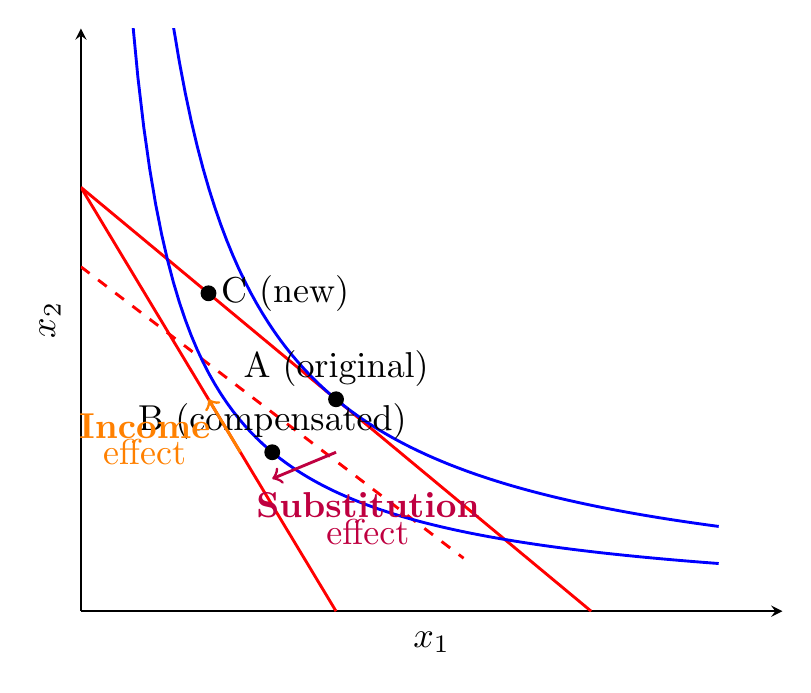
\begin{tikzpicture}[scale=1.3]
\begin{axis}[
    axis lines=left,
    xlabel={$x_1$},
    ylabel={$x_2$},
    xmin=0, xmax=11,
    ymin=0, ymax=11,
    xtick=\empty,
    ytick=\empty,
    domain=0.8:10,
    samples=100
]
% Original budget
\addplot[red, thick] coordinates {(0,8) (8,0)};
% New budget (p1 increases)
\addplot[red, thick] coordinates {(0,8) (4,0)};
% Compensated budget
\addplot[red, dashed, thick] coordinates {(0,6.5) (6,1)};
% IC curves
\addplot[blue, thick] {16/x};
\addplot[blue, thick] {9/x};
% Points
\filldraw[black] (axis cs:4,4) circle (2pt);
\node[above] at (axis cs:4,4) {A (original)};
\filldraw[black] (axis cs:3,3) circle (2pt);
\node[above] at (axis cs:3,3) {B (compensated)};
\filldraw[black] (axis cs:2,6) circle (2pt);
\node[right] at (axis cs:2,6) {C (new)};
% Arrows
\draw[->,thick,purple] (axis cs:4,3) -- (axis cs:3,2.5);
\node[purple] at (axis cs:4.5,2) {\textbf{Substitution}};
\node[purple] at (axis cs:4.5,1.5) {effect};
\draw[->,thick,orange] (axis cs:2.5,3) -- (axis cs:2,4);
\node[orange] at (axis cs:1,3.5) {\textbf{Income}};
\node[orange] at (axis cs:1,3) {effect};
\end{axis}
\end{tikzpicture}
\end{center}

\begin{intuition}
When $p_1$ rises:
\begin{itemize}
    \item \textbf{Substitution effect (A→B):} Good 1 is now relatively more expensive, so you substitute toward good 2. Move along the IC to the new price ratio. This ALWAYS reduces $x_1$.
    \item \textbf{Income effect (B→C):} You're effectively poorer (your money doesn't stretch as far). If $x_1$ is a normal good, you buy less. If it's inferior, you might buy more!
\end{itemize}
\end{intuition}

\begin{steps}
\textbf{How to calculate:}
\begin{enumerate}
    \item Find original bundle at $(p_1, p_2, m)$: call it $A$
    \item Calculate utility at $A$: $\bar{u} = u(A)$
    \item Find compensated bundle: minimize spending to reach $\bar{u}$ at new prices $(p_1', p_2, m)$. Call it $B$.
    \item Substitution effect = $B - A$
    \item Find new actual bundle at $(p_1', p_2, m)$: call it $C$
    \item Income effect = $C - B$
    \item Total effect = $C - A$ = sub + income
\end{enumerate}
\end{steps}

\begin{warning}
For \textbf{perfect complements}, there is NO substitution effect (you can't substitute - you need them in fixed proportions). The entire change is income effect!

For \textbf{quasilinear}, there is NO income effect for the quasilinear good (at interior solutions).
\end{warning}

\section{Uncertainty \& Risk}

\subsection{Expected Utility Theory}

You face a lottery with outcomes $c_1, c_2, \ldots$ with probabilities $p_1, p_2, \ldots$

\textbf{Expected Utility:}
$$EU = p_1 u(c_1) + p_2 u(c_2) + \cdots$$

\begin{intuition}
You don't just care about the average outcome - you care about the utility of each outcome. If you're risk-averse, bad outcomes hurt more than good outcomes help (in utility terms).
\end{intuition}

\subsection{Risk Aversion}

\begin{center}
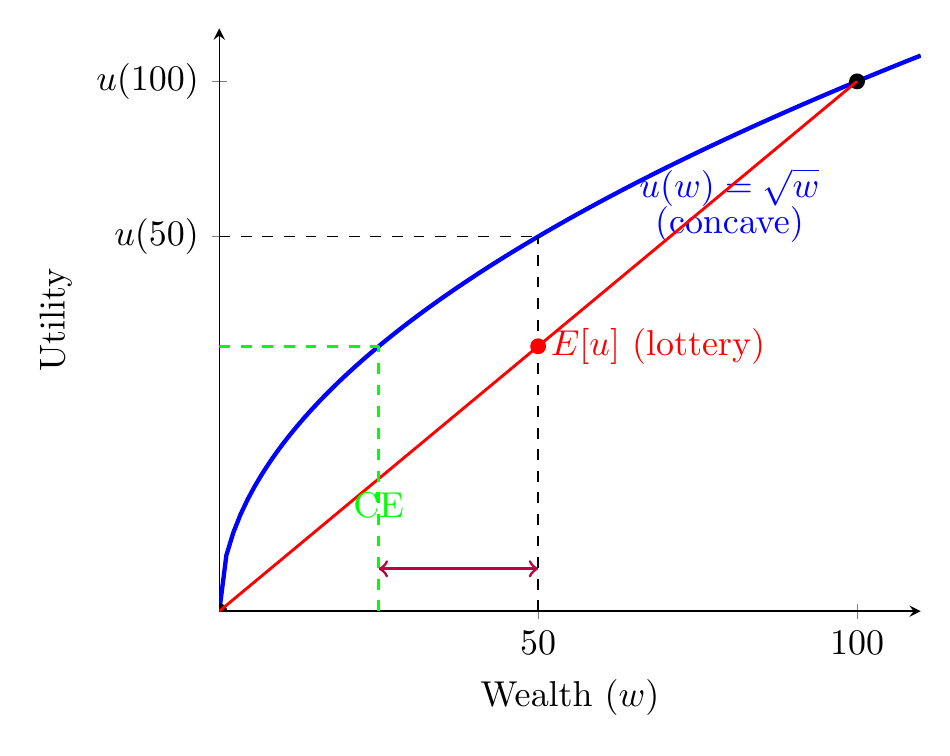
\begin{tikzpicture}[scale=1.3]
\begin{axis}[
    axis lines=left,
    xlabel={Wealth ($w$)},
    ylabel={Utility},
    xmin=0, xmax=110,
    ymin=0, ymax=11,
    xtick={50,100},
    ytick={7.07,10},
    yticklabels={$u(50)$,$u(100)$},
    domain=0:110,
    samples=100
]
\addplot[blue, very thick] {sqrt(x)};
\node[blue] at (axis cs:80,8) {$u(w) = \sqrt{w}$};
\node[blue] at (axis cs:80,7.3) {(concave)};
% Lottery outcomes
\filldraw (axis cs:0,0) circle (2pt);
\filldraw (axis cs:100,10) circle (2pt);
% Expected value
\draw[dashed] (axis cs:50,0) -- (axis cs:50,7.07);
\draw[dashed] (axis cs:0,7.07) -- (axis cs:50,7.07);
% Chord
\draw[red, thick] (axis cs:0,0) -- (axis cs:100,10);
\filldraw[red] (axis cs:50,5) circle (2pt);
\node[red, right] at (axis cs:50,5) {$E[u]$ (lottery)};
% CE
\draw[dashed,green,thick] (axis cs:0,5) -- (axis cs:25,5);
\draw[dashed,green,thick] (axis cs:25,0) -- (axis cs:25,5);
\node[green] at (axis cs:25,2) {CE};
% Arrows
\draw[<->,thick,purple] (axis cs:25,0.8) -- (axis cs:50,0.8);
\node[purple,below] at (axis cs:37.5,0) {Risk Premium};
\end{axis}
\end{tikzpicture}
\end{center}

\begin{intuition}
\textbf{Risk averse:} Your utility function is concave (bends down). This means:
\begin{itemize}
    \item You prefer \$50 for sure over a 50-50 gamble of \$0 or \$100
    \item Even though the expected value is the same (\$50), the expected utility of the gamble is lower
    \item You'd pay to avoid risk (insurance!)
\end{itemize}
\end{intuition}

\textbf{Key formulas:}
\begin{itemize}
    \item \textbf{Certainty Equivalent (CE):} The sure amount worth the same as the gamble: $u(CE) = E[u]$
    \item \textbf{Risk Premium (RP):} How much you'd pay to avoid the risk: $RP = E[w] - CE$
\end{itemize}

\begin{example}
\textbf{Problem:} You have $u(w) = \sqrt{w}$. You face a 50-50 lottery of \$0 or \$100.

\textbf{Solution:}
\begin{enumerate}
    \item Expected value: $E[w] = 0.5(0) + 0.5(100) = 50$
    \item Expected utility: $E[u] = 0.5\sqrt{0} + 0.5\sqrt{100} = 0 + 5 = 5$
    \item Certainty equivalent: $u(CE) = 5 \Rightarrow \sqrt{CE} = 5 \Rightarrow CE = 25$
    \item Risk premium: $RP = 50 - 25 = 25$
\end{enumerate}

\textbf{Interpretation:} The lottery is worth only \$25 to you (even though it has an expected value of \$50). You'd pay up to \$25 to avoid this risk!
\end{example}

\subsection{Insurance Problem}

You have wealth $w$ and might lose $D$ with probability $\pi$. Insurance costs $q$ per dollar of coverage $K$.

\textbf{Your wealth in each state:}
\begin{itemize}
    \item No loss (prob $1-\pi$): $w - qK$
    \item Loss (prob $\pi$): $w - D - qK + K = w - D + K(1-q)$
\end{itemize}

\textbf{Expected utility:}
$$EU = (1-\pi) u(w - qK) + \pi u(w - D + K(1-q))$$

\begin{center}
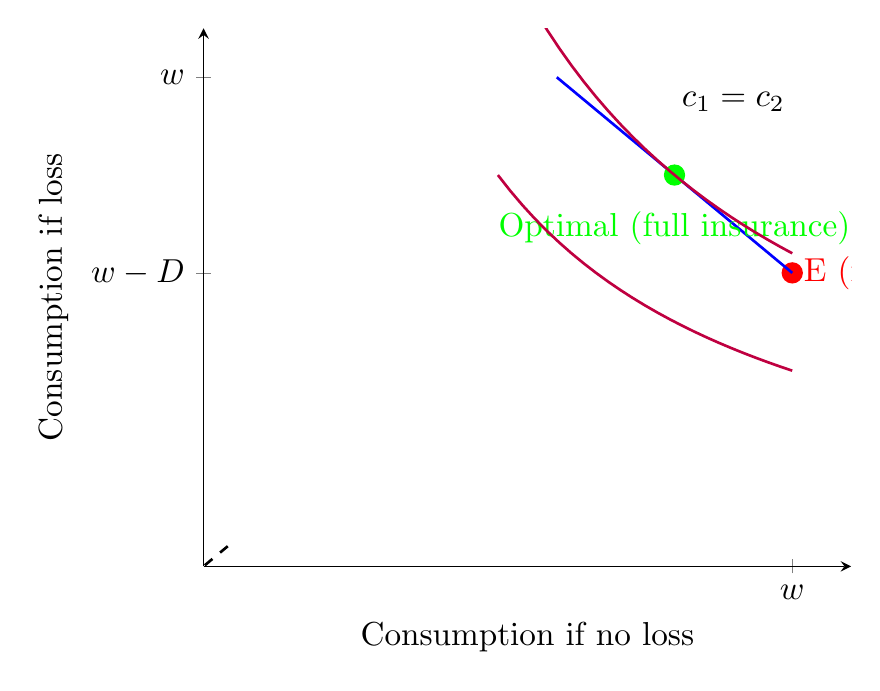
\begin{tikzpicture}[scale=1.2]
\begin{axis}[
    axis lines=left,
    xlabel={Consumption if no loss},
    ylabel={Consumption if loss},
    xmin=0, xmax=110,
    ymin=0, ymax=110,
    xtick={100},
    ytick={60,100},
    yticklabels={$w-D$,$w$},
    xticklabels={$w$},
]
% 45-degree line
\addplot[dashed, thick] {x};
\node at (axis cs:90,95) {$c_1 = c_2$};
% Initial endowment
\filldraw[red] (axis cs:100,60) circle (3pt);
\node[red,right] at (axis cs:100,60) {E (no insurance)};
% Budget line (fair insurance)
\addplot[blue, thick] coordinates {(100,60) (60,100)};
% Optimum (full insurance with fair prices)
\filldraw[green] (axis cs:80,80) circle (3pt);
\node[green,below] at (axis cs:80,75) {Optimal (full insurance)};
% IC curves
\addplot[purple, thick, domain=50:100] {4000/x};
\addplot[purple, thick, domain=50:100] {6400/x};
\end{axis}
\end{tikzpicture}
\end{center}

\begin{intuition}
\textbf{With fair insurance ($q = \pi$):} A risk-averse person buys full insurance ($K = D$). This makes consumption the same in both states - no uncertainty! The budget line is drawn so it passes through the 45° line, where you're fully insured.

\textbf{With unfair insurance ($q > \pi$):} You buy partial insurance - some, but not full, coverage.
\end{intuition}

\begin{steps}
\textbf{How to solve:}
\begin{enumerate}
    \item Write expected utility as function of $K$
    \item Take derivative: $\frac{dEU}{dK} = 0$
    \item This gives: $(1-\pi) u'(w-qK) \cdot (-q) + \pi u'(w-D+K(1-q)) \cdot (1-q) = 0$
    \item Simplify to find $K^*$
    \item For fair insurance, this yields $K^* = D$ (full insurance)
\end{enumerate}
\end{steps}

\section{General Equilibrium: Markets Clear}

\subsection{Edgeworth Box}

Two consumers (A and B), two goods (1 and 2), total endowments $(E_1, E_2)$.

\begin{center}
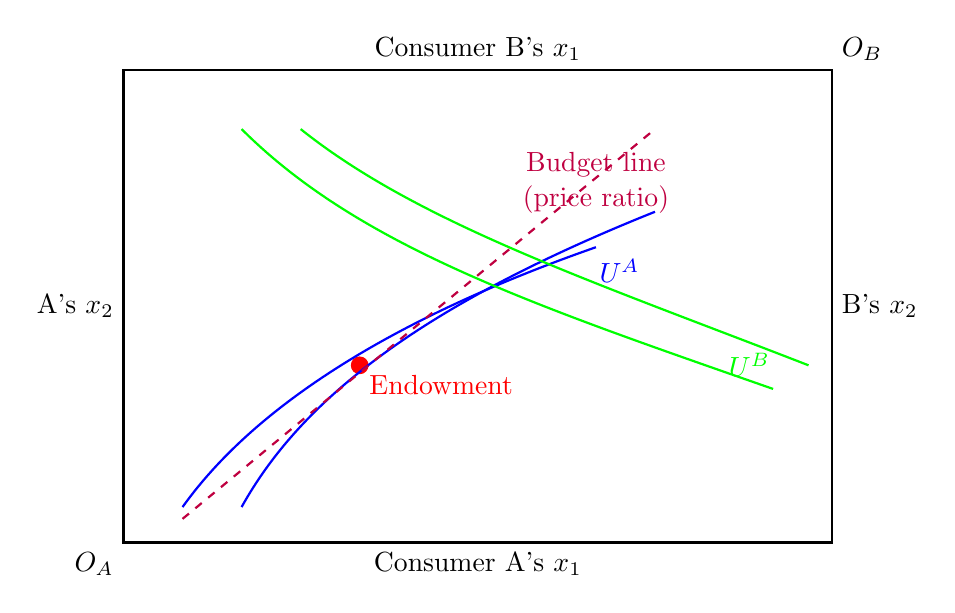
\begin{tikzpicture}[scale=1.5]
% Box
\draw[thick] (0,0) rectangle (6,4);
% Labels
\node[below] at (3,0) {Consumer A's $x_1$};
\node[left] at (0,2) {A's $x_2$};
\node[above] at (3,4) {Consumer B's $x_1$};
\node[right] at (6,2) {B's $x_2$};
% Origins
\node[below left] at (0,0) {$O_A$};
\node[above right] at (6,4) {$O_B$};
% Endowment
\filldraw[red] (2,1.5) circle (2pt);
\node[red,below right] at (2,1.5) {Endowment};
% ICs for A (from bottom-left)
\draw[blue, thick] (0.5,0.3) .. controls (1,1) and (2,1.8) .. (4,2.5);
\draw[blue, thick] (1,0.3) .. controls (1.5,1.2) and (2.5,2) .. (4.5,2.8);
\node[blue] at (4.2,2.3) {$U^A$};
% ICs for B (from top-right, reading backwards)
\draw[green, thick] (1,3.5) .. controls (2,2.5) and (3.5,2) .. (5.5,1.3);
\draw[green, thick] (1.5,3.5) .. controls (2.5,2.7) and (4,2.2) .. (5.8,1.5);
\node[green] at (5.3,1.5) {$U^B$};
% Budget line through endowment
\draw[purple, thick, dashed] (0.5,0.2) -- (4.5,3.5);
\node[purple] at (4,3.2) {Budget line};
\node[purple] at (4,2.9) {(price ratio)};
\end{tikzpicture}
\end{center}

\begin{intuition}
The Edgeworth box shows all possible allocations. The width is total $x_1$, the height is total $x_2$. A reads from the bottom-left corner, B reads from the top-right (flipped). Any point in the box is a feasible allocation (adding up to total endowments).
\end{intuition}

\subsection{Competitive Equilibrium}

\textbf{Equilibrium conditions:}
\begin{enumerate}
    \item Each consumer maximizes utility given budget: $p \cdot x^i = p \cdot e^i$
    \item Markets clear: $x_1^A + x_1^B = E_1$ and $x_2^A + x_2^B = E_2$
\end{enumerate}

\begin{steps}
\textbf{How to solve:}
\begin{enumerate}
    \item Normalize $p_2 = 1$ (so all prices are relative to good 2)
    \item Calculate each person's income: $m^A = p_1 e_1^A + e_2^A$ (value of their endowment)
    \item Solve each person's UMP to get demands: $x_1^A(p_1)$ and $x_1^B(p_1)$
    \item Market clearing: $x_1^A(p_1) + x_1^B(p_1) = E_1$
    \item Solve for equilibrium price $p_1^*$
    \item Plug back to get equilibrium allocations
    \item Verify: $x_2^A, x_2^B \geq 0$ (no one demands negative amounts)
\end{enumerate}
\end{steps}

\begin{example}
\textbf{Problem:} 2 consumers with Cobb-Douglas utilities:
\begin{itemize}
    \item A: $u^A = x_1^{0.5} x_2^{0.5}$, endowment $(4, 0)$
    \item B: $u^B = x_1^{0.5} x_2^{0.5}$, endowment $(0, 4)$
\end{itemize}

\textbf{Solution:}
\begin{enumerate}
    \item Set $p_2 = 1$, so prices are $(p_1, 1)$
    \item Incomes: $m^A = 4p_1$, $m^B = 4$
    \item CD demands: spend half on each good
    \begin{itemize}
        \item $x_1^A = \frac{m^A/2}{p_1} = \frac{2p_1}{p_1} = 2$
        \item $x_1^B = \frac{m^B/2}{p_1} = \frac{2}{p_1}$
    \end{itemize}
    \item Market clearing: $2 + \frac{2}{p_1} = 4$
    \item $\frac{2}{p_1} = 2 \Rightarrow p_1^* = 1$
    \item Equilibrium: $(p_1, p_2) = (1, 1)$
    \item Allocations: $x^A = (2, 2)$, $x^B = (2, 2)$
\end{enumerate}

They split everything equally! (Makes sense - identical preferences, symmetric endowments.)
\end{example}

\subsection{Pareto Efficiency}

An allocation is \textbf{Pareto efficient (PE)} if you can't make someone better off without making someone else worse off.

\begin{intuition}
At a PE allocation, the indifference curves of A and B are tangent: $MRS^A = MRS^B$. If they weren't tangent, there would be a "lens" between the curves where both could be better off.
\end{intuition}

\textbf{Key Results:}
\begin{itemize}
    \item \textbf{First Welfare Theorem:} Every competitive equilibrium is Pareto efficient
    \item \textbf{Second Welfare Theorem:} Any Pareto efficient allocation can be achieved as a competitive equilibrium (with the right redistribution of endowments)
\end{itemize}

\section{Quick Problem-Solving Guide}

\begin{steps}
\textbf{For utility maximization:}
\begin{enumerate}
    \item Identify the utility function type (CD, PC, PS, QL, or general)
    \item If CD: use the shortcut (spend fraction $a/(a+b)$ on each good)
    \item If PC: set $ax_1 = bx_2$ and use budget
    \item If PS: compare $a/p_1$ vs $b/p_2$ and buy all of the better one
    \item Otherwise: $MRS = p_1/p_2$ and budget constraint
    \item Always check: are your answers non-negative? If not, corner solution!
\end{enumerate}
\end{steps}

\begin{steps}
\textbf{For income/substitution effects:}
\begin{enumerate}
    \item Original bundle ($A$) at old prices
    \item Calculate original utility
    \item Compensated bundle ($B$): new prices, old utility (minimize cost or stay on same IC)
    \item New bundle ($C$) at new prices
    \item Sub effect = $B - A$ (always negative for own price)
    \item Income effect = $C - B$ (sign depends on normal/inferior)
\end{enumerate}
\end{steps}

\begin{steps}
\textbf{For expected utility:}
\begin{enumerate}
    \item List all outcomes and probabilities
    \item Write $EU = \sum p_i u(c_i)$
    \item If finding optimal choice (insurance, portfolio): take FOC, set = 0, solve
    \item If finding CE: set $u(CE) = EU$ and solve for CE
    \item If finding RP: $RP = E[w] - CE$
\end{enumerate}
\end{steps}

\begin{warning}
\textbf{Common traps:}
\begin{itemize}
    \item Forgetting to check $x_i \geq 0$ (corner solutions!)
    \item Mixing up substitution effect direction (always buy LESS of the good that got more expensive)
    \item Using arbitrary transforms on vNM utility (only affine transforms allowed!)
    \item Confusing variance ($\sigma^2$) with std deviation ($\sigma$)
    \item Forgetting that PC has zero substitution effect
\end{itemize}
\end{warning}

\end{document}
